\documentclass{article}
\usepackage{arxiv}

\usepackage[utf8]{inputenc} % allow utf-8 input
\usepackage[math]{anttor}   % Antykwa torunska
\usepackage[T1]{fontenc}    % use 8-bit T1 fonts
\usepackage{hyperref}       % hyperlinks
\usepackage{url}            % simple URL typesetting
\usepackage{booktabs}       % professional-quality tables
\usepackage{amsfonts}       % blackboard math symbols
\usepackage{nicefrac}       % compact symbols for 1/2, etc.
\usepackage{microtype}      % microtypography
\usepackage{graphicx}       % adding figures
\usepackage{gensymb}        % general symbols
\usepackage{wasysym}        % more symbols like permile
\usepackage{changepage}

\title{Protokół komunikacji Advantech-TTControl}

\begin{document}
\maketitle
\author{Agribot team}

\section{Wstęp}
W celu łatwiejszego zrozumienia opisywanego protokołu komunikacji miedzy sterownikiem TTControl i komputerem Advantech, zalecane jest przeczytanie niniejszej sekcji. 
\subsection{Możliwe stany robota Agribot}

\begin{center}
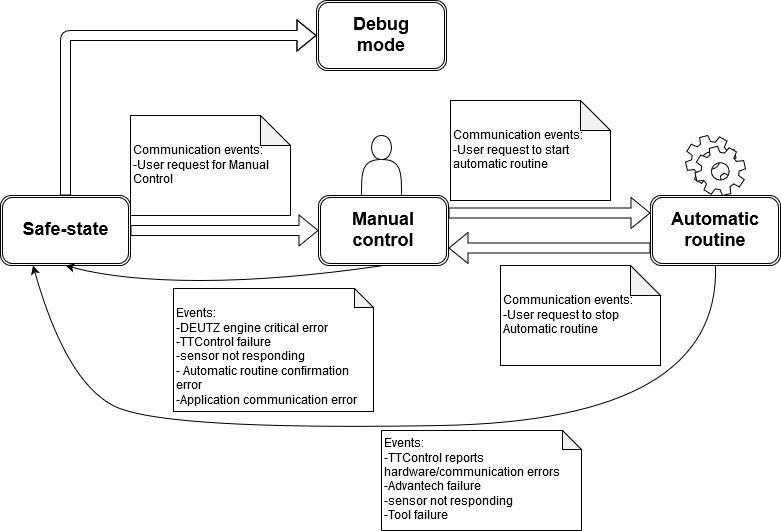
\includegraphics[scale=0.5]{AgribotStates.jpg}
\end{center}{}

Agribot może znajdować się w jednym z czterech stanów:
\begin{itemize}
    \item Safe-state
    \item Manual control
    \item Automatic routine 
    \item Debug mode
\end{itemize}

Domyślnie robot znajduje się w stanie Safe-state, który to utrzymuje robota w bezruchu, w oczekiwaniu na użytkownika lub w wypadku awarii wyłącza silnik. Na żądanie użytkownika, za pośrednictwem aplikacji, można przejść ze stanu Safe-state do Manual control. W wypadku błędów robota lub niestabilnej komunikacji (np: zbyt duże odstępy między kolejnymi ramkami Hearbeat, lub zgubienie jednej z ramek Hearbeat) robot wraca do stanu Safe-state. Ze stanu Manual control, użytkownik może wprowadzić robota w stan Automatic routine. Jeśli konfiguracja wymagana do automatycznej pracy robota nie została przeprowadzana poprawnie, robot wróci do stanu Manual Control. Użytkownik może z poziomu aplikacji zatrzymać automatyczną pracę i wrócić do stanu Manual control. W wypadku wystąpienia błędów hardwear robota lub komunikacji między TTControl a Advantech, robot przechodzi w stan Safe-state.

\subsection{Wykorzystywana struktura adresów CAN}
Protokół komunikacji między TTControl i Advantech jest oparty na protokole SAE J1939. Poniżej znajduje się struktura 29-bitowego adresu ramki CAN.
\begin{center}
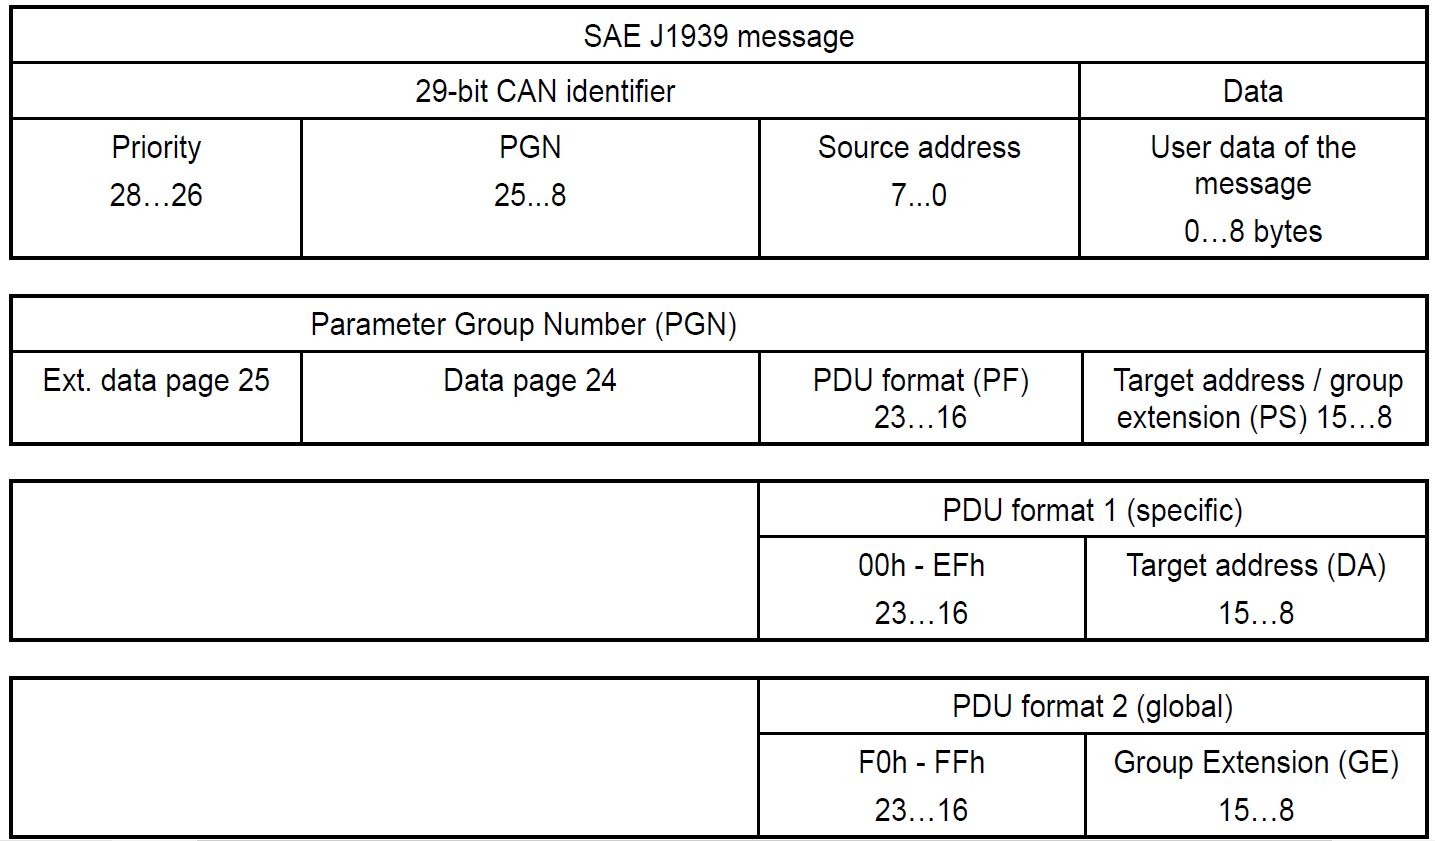
\includegraphics[scale=0.5]{SAEJ1939Format.JPG}
\end{center}{}

W protokole SAE J1939, adres ramki CAN określa sposób interpretacji danych i ich przeznaczenie, a także nadawcę i odbiorce. 3 bity Priority określają priorytet wiadomości, gdzie 0 to najwyższy priorytet wiadomości. Następnie PGN określa funkcję ramki/sposób interpretacji danych a także odbiorcę (broadcast lub konkretne urządzenie w sieci). Każde urządzenie ma przypisany swój adres sieciowy (0x00-0xFF), który w przypadku wykonywania każdej transmisji urządzenie umieszcza na końcu  29-bitowego adresu. TTControl posiada adres 100 (0x64), a Advantech posiada adres sieciowy 200 (0xC8).\\

\section{Opis protokołu i wymiany danych}
\subsection{Procedura Handshake}
Komputer Advantech inicjuje nawiązanie połączenia z TTControl, a następnie czeka na odpowiedź od TTControl. TTControl po otrzymaniu wiadomości, odpowiada Advantechowi ramką potwierdzająca otrzymanie żądania połączenia.\\

Advantech do TTControl\\
Priority: 0x00, PGN: 0x0EF64, Source adres: 0xC8\\
\begin{left}
\begin{tabular}{ |p{2cm}|p{1.5cm}|} 
 \hline
 CAN ID & BYTE 0\\ \hline
 &\\
 0x00EF64C8 & 0x10\\ 
 \hline
\end{tabular}
\end{left}\\

TTControl do Advantech\\
Priority: 0x00, PGN: 0x0EFC8, Source adres: 0x64\\
\begin{left}
\begin{tabular}{ |p{2cm}|p{1.5cm}|} 
 \hline
 CAN ID & BYTE 0\\ \hline
 &\\
 0x00EFC864 & 0x10\\ 
 \hline
\end{tabular}
\end{left}\\

Jeśli sterownik TTControl nie odpowiada na ramkę inicjalizującą, Advantech spróbuje ponownie po upływie 5 sekund. 

\subsection{Rutyna Hearbeat}
Rutyna ta jest wykonywana między Advantechem i TTControl w regularnym interwale czasowym krótszym od 200 ms. Jeśli nie zostanie ona poprawnie wykonana, sterowanie zostaje przerwane i robot wraca do stanu Safe-state. Procedura rozpoczyna się od wysłania przez Advantech pierwszej ramki Hearbeat, po której oczekuje odpowiedniej odpowiedzi od TTControl. Jeśli którykolwiek ze sterowników prześlę złą odpowiedź na Hearbeat lub zrobi to w czasie dłuższym niż 200 ms, połączenie zostaje przerwane i robot wchodzi w stan Safe-state.\\

Advantech do TTControl\\
Priority: 0x00, PGN: 0x0EF64, Source adres: 0xC8 Interval: 200ms\\
\begin{left}
\begin{tabular}{ |p{2cm}|p{1.5cm}|} 
 \hline
 CAN ID & BYTE 0 \\ \hline
 & \\
 0x00FFDFC8 & HB\_ID\\ 
 \hline
\end{tabular}
\end{left}\\


TTControl do Advantech\\
Priority: 0x00, PGN: 0x0EF64, Source adres: 0x64 Interval: 200ms\\
\begin{left}
\begin{tabular}{ |p{2cm}|p{1.5cm}|} 
 \hline
 CAN ID & BYTE 0\\ \hline
 & \\
 0x00FFDF64 & HB\_ID\\ 
 \hline
\end{tabular}
\end{left}\\

HB\_ID to aktualny indeks Hearbeat, sterownik który otrzymał HB\_ID o danym numerze powinien inkrementować jego wartość i przesłac z powrotem. Przykładowo, Advantech zaczyna od HB\_ID=0, wysyła HB i oczekuje HB\_ID=1, TTControl otrzymuje wiadomość, inkrementuje HB\_ID, wysyła wiadomość z HB\_ID=1 i oczekuje na wiadomość z wartością HB\_ID=2.

\subsection{Wejscie w tryb automatic routine i powrot do stanu safe-state }

Komputer TTControl po otrzymaniu ramki uruchomienia automatycznej pracy, przechodzi w stan automatycznej kontroli pod warunkiem, ze agribot nie znajduje sie aktualnie w manualnym sterowaniu. Bajt command moze przyjac wartosci:
\begin{itemize}
\item 0 - wejdz w stan safe state
\item 1 - wejdz w stan automatycznego sterowania
\end{itemize}

Advantech do TTControl\\
Priority: 0x00, PGN: 0x0EF64, Source adres: 0xC8\\
\begin{left}
\begin{tabular}{ |p{2cm}|p{1.5cm}|p{2.0cm}|p{2.0cm}|}  
 \hline
 CAN ID & BYTE 0 & BYTE 1 & BYTE 2\\ \hline
 & & &\\
 0x00EFC864 & 0x20 & 0x64 & Command\\ 
 \hline
\end{tabular}
\end{left}\\

Mozliwe wartosci resultatu:
\begin{itemize}
\item 0 - robot wszedl w stan automatyczny
\item 255 - stan automatyczny niemozliwy, gdyz robot znajduje sie w stanie manual
\end{itemize}

Advantech do TTControl\\
Priority: 0x00, PGN: 0x0EFC8, Source adres: 0x64\\
\begin{left}
\begin{tabular}{ |p{2cm}|p{1.5cm}|p{2.0cm}|p{2.0cm}|}   
 \hline
 CAN ID & BYTE 0 & BYTE 1 & BYTE 2 \\ \hline
 & & &\\
 0x00EF64C8 & 0x20 & 0x64 & Result\\ 
 \hline
\end{tabular}
\end{left}\\


\subsection{Sygnały sterowania}
Wszystkie sygnały sterowania posiadają time-out rozkazu. Jeśli przez 300 ms TTControl nie otrzyma sygnału sterowania, TTControl przestaje podawać sygnał na wyjścia i efektory zatrzymują się. 
\subsubsection{Sterowanie wózkami}

Advantech do TTControl\\
Priority: 0x00, PGN: 0x0FFD0, Source adres: 0xC8, Interval: 200ms\\
\begin{left}
\begin{tabular}{ |p{2cm}|p{1.5cm}|p{1.5cm}|p{1.5cm}|p{1.5cm}|p{1.5cm}|p{1.5cm}|p{1.5cm}|p{1.5cm}|} 
 \hline
 CAN ID & BYTE 0 & BYTE 1 & BYTE 2 & BYTE 3 & BYTE 4 & BYTE 5 & BYTE 6 & BYTE 7\\ \hline
 & & & & & & & &\\
0x00FFD0C8 & F\_LIN\_H & F\_LIN\_L & F\_ANG\_H & F\_ANG\_H & B\_LIN\_H & B\_LIN\_L & B\_ANG\_H & B\_ANG\_L\\ 
 \hline
\end{tabular}
\end{left}\\

TTControl do Advantech\\
Priority: 0x00, PGN: 0x0FFD0, Source adres: 0x64, Interval: 200ms\\
\begin{left}
\begin{tabular}{ |p{2cm}|p{1.5cm}|p{1.5cm}|p{1.5cm}|p{1.5cm}|p{1.5cm}|p{1.5cm}|p{1.5cm}|p{1.5cm}|} 
 \hline
 CAN ID & BYTE 0 & BYTE 1 & BYTE 2 & BYTE 3 & BYTE 4 & BYTE 5 & BYTE 6 & BYTE 7\\ \hline
 & & & & & & & &\\
0x00FFD064 & F\_LIN\_H & F\_LIN\_L & F\_ANG\_H & F\_ANG\_H & B\_LIN\_H & B\_LIN\_L & B\_ANG\_H & B\_ANG\_L\\ 
 \hline
\end{tabular}
\end{left}\\

\subsubsection{Sterowanie geometrią delt}
Ramka wysyłana z Advantecha do TTControl zawiera 2 bajty, bajt ustawiony na 0x01 oznacza wysuniecie siłownika gąsienicy, a o 0x00 oznacza schowanie go. Bajt FRONT\_GEOM to komenda dla wózka przedniego, a BACK\_GEOM jest dla wózka tylnego. Ramka stanu wózków jest wysyłana cyklicznie i zawiera aktualne wysuniecie wózków.\\

Advantech do TTControl\\
Priority: 0x00, PGN: 0x0FFDC, Source adres: 0xC8, Interval: when requested \\
\begin{left}
\begin{tabular}{ |p{2cm}|p{2.5cm}|p{2.5cm}|} 
 \hline
 CAN ID & BYTE 0 & BYTE 1 \\ \hline
 & & \\
0x00FFDCC8 & FRONT\_GEOM & BACK\_GEOM \\ 
 \hline
\end{tabular}
\end{left}\\

TTControl do Advantech\\
Priority: 0x00, PGN: 0x0FFDC, Source adres: 0x64, Interval: 200 ms \\
\begin{left}
\begin{tabular}{ |p{2cm}|p{2.5cm}|p{2.5cm}|} 
 \hline
 CAN ID & BYTE 0 & BYTE 1 \\ \hline
 & & \\
0x00FFDC64 & FRONT\_GEOM & BACK\_GEOM \\ 
 \hline
\end{tabular}
\end{left}\\

\subsubsection{Konfiguracja parametrów}
Każda z ramek na pierwszym bajcie posiada specyfikacje typu rami, czyli jakie parametry ona zmienia.
Pierwsza ramka odpowiada za parametry sygnałów sterowania i sygnałów wejściowych z enkoderow. Lista parametrow tej ramki prezentuje sie nastepujaco:
\begin{itemize}
\item PAR\_IND -- w przypadku ramki parametrow sygnalu wynosi on 0
\item DITT\_T -- to okres wymuszonego drgania cewki (ditter) wyrazony w X*4 ms. Mimalna wartosc tego parametru to 1 a maksymalna to 256. Oznacza to ze minimalny okres sygnalu ditter cewki wynosi 4 ms a maksymalny 1024 ms. Domyslnie okres ten wynosi 16 ms (wartość parametru 4).
\item DITT\_A -- to procent maksymalnej wartosci sygnalu sterowania o jaki wacha sie ditter (amplituda ditter). Moze przyjac wartosci od 0 \permil do 3000 \permil. Domyslnie wynosi on 1000 \permil. 
\item ENC\_T -- to okres pomiaru predkosci enkoderow wyrazony w wielokrotnosciach 50 ms, i moze przyjmowac wartosci od 1 do 20. Mniejsza wartosc tego parametru daje wieksza dokladnosc pomiaru ale zwieksza podatnosc na zaklocenia, wieksza wartosc zmniejsza czulosc ale wygladza sygnal wejsciowy. Domyslnie ustawiony na 6, czyli okres pomiaru predkosci wynosi 6*50 ms  = 300 ms.  
\end{itemize}

Advantech do TTControl, PAR\_IND = 0\\
Priority: 0x00, PGN: 0x0FFDB, Source adres: 0xC8 \\
\begin{left}
\begin{tabular}{ |p{2cm}|p{1.35cm}|p{1.2cm}|p{1.50cm}|p{1.50cm}|p{1.35cm}|p{1.35cm}|p{1.35cm}|p{1.35cm}|p{1.35cm}|} 
 \hline
 CAN ID & BYTE 0 & BYTE 1 & BYTE 2 & BYTE 3 & BYTE 4 & BYTE 5 & BYTE 6 & BYTE 7 \\ \hline
 & & & & & & & &\\
0x00FFDBC8 & PAR\_IND & DITT\_T & DITT\_A\_L & DITT\_A\_H  & ENC\_T & 0xFF & 0xFF & 0xFF\\
 \hline
\end{tabular}
\end{left}\\

Drugi typ ramki to parametry regulatora predkosci przedniego wozka. Zawiera ona nastepujace parametry. 
\begin{itemize}
    \item KP\_T -- wzmocnienie czlonu proporcjonalnego translacyjnej czesci regulatora (czyli predkosci liniowej), zapisane razy 10000, w celu przeslania czesci dziesietnej parametru.
    \item KI\_T -- wzmocnienie czlonu calkujacego translacyjnej czesci regulatora (czyli predkosci liniowej), zapisane razy 10000, w celu przeslania czesci dziesietnej parametru.
    \item KD\_T -- wzmocnienie czlonu rozniczkowego translacyjnej czesci regulatora (czyli predkosci liniowej), zapisane razy 100, w celu przeslania czesci dziesietnej parametru.
    \item ACC\_T -- przyspieszenie punktu zadanego (SP), rozdzielczosc to 0.001, czyli nalezy przeslac zadana wartosc przemnozona przez 1000, przykladowo 0.07 zostanie zapisane jako 70. Wartosc przyspieszenia jest dodawana do aktualnej wartosci SP regulatora co 100 ms.
\end{itemize}

Advantech do TTControl, PAR\_IND  = 1, 3\\
Priority: 0x00, PGN: 0x0FFDB, Source adres: 0xC8 \\
\begin{left}
\begin{tabular}{ |p{2cm}|p{1.35cm}|p{1.2cm}|p{1.50cm}|p{1.50cm}|p{1.35cm}|p{1.4cm}|p{1.4cm}|p{1.35cm}|p{1.6cm}|} 
 \hline
 CAN ID & BYTE 0 & BYTE 1 & BYTE 2 & BYTE 3 & BYTE 4 & BYTE 5 & BYTE 6 & BYTE 7 \\ \hline
 & & & & & & & &\\
0x00FFDBC8 & PAR\_IND & KP\_T\_L & KP\_T\_H & KI\_T\_L & KI\_T\_H & KD\_T & ACC\_T\_L & ACC\_T\_H  \\
 \hline
\end{tabular}
\end{left}\\

Trzeci typ ramki to kolejne parametry regulatora predkosci przedniego wozka. Zawiera ona nastepujace parametry. 
\begin{itemize}
    \item KP\_R -- wzmocnienie czlonu proporcjonalnego czesci rotacyjnej regulatora (czyli predkosci katowej), zapisane razy 10000, w celu przeslania czesci dziesietnej parametru.
    \item KI\_R -- wzmocnienie czlonu calkujacego czesci rotacyjnej regulatora (czyli predkosci katowej), zapisane razy 10000, w celu przeslania czesci dziesietnej parametru.
    \item KD\_R -- wzmocnienie czlonu rozniczkowego czesci rotacyjnej regulatora (czyli predkosci katowej), zapisane razy 100, w celu przeslania czesci dziesietnej parametru.
    \item ACC\_R -- przyspieszenie punktu zadanego (SP), rozdzielczosc to 0.001, czyli nalezy przeslac zadana wartosc przemnozona przez 1000, przykladowo 0.07 zostanie zapisane jako 70. Wartosc przyspieszenia jest dodawana do aktualnej wartosci SP regulatora co 100 ms.
\end{itemize}

Advantech do TTControl, PAR\_IND  = 2, 4\\
Priority: 0x00, PGN: 0x0FFDB, Source adres: 0xC8 \\
\begin{left}
\begin{tabular}{ |p{2cm}|p{1.35cm}|p{1.2cm}|p{1.50cm}|p{1.50cm}|p{1.35cm}|p{1.4cm}|p{1.4cm}|p{1.35cm}|p{1.35cm}|} 
 \hline
 CAN ID & BYTE 0 & BYTE 1 & BYTE 2 & BYTE 3 & BYTE 4 & BYTE 5 & BYTE 6 & BYTE 7 \\ \hline
 & & & & & & & &\\
0x00FFDBC8 & PAR\_IND & KP\_R\_L & KP\_R\_H & KI\_R\_L & KI\_R\_H & KD\_R & ACC\_R\_L & ACC\_R\_H \\
 \hline
\end{tabular}
\end{left}\\

Ramki dla tylniego wozka, wygladaja identycznie jak ramki wozka przedniego, pelnia te same funckje i roznia sie tylko wartosciami bajtu specyfikacji, czyli: 
\begin{itemize}
    \item PAR\_IND  = 1 to ramka przedniego, dla tylniego PAR\_IND  = 3
    \item PAR\_IND  = 2 to ramka przedniego, dla tylniego PAR\_IND  = 4
\end{itemize}

Czwarty typ ramki to konfiguracja parametrow regulatorow PID strerujacych pradem cewek dla poszczegolnych gasienic.

Advantech do TTControl, PAR\_IND  = 5, 7, 9, 11\\
Priority: 0x00, PGN: 0x0FFDB, Source adres: 0xC8 \\
\begin{left}
\begin{tabular}{ |p{2cm}|p{1.35cm}|p{1.2cm}|p{1.50cm}|p{1.50cm}|p{1.35cm}|p{1.4cm}|p{1.4cm}|p{1.35cm}|p{1.35cm}|} 
 \hline
 CAN ID & BYTE 0 & BYTE 1 & BYTE 2 & BYTE 3 & BYTE 4 & BYTE 5 & BYTE 6 & BYTE 7 \\ \hline
 & & & & & & & &\\
0x00FFDBC8 & PAR\_IND & KP\_L & KP\_H & KI\_L & KI\_H & KD\_L & KD\_H & 0xFF \\
 \hline
\end{tabular}
\end{left}\\

Ramki dla poszczegolnych gasienic posiadaja nastepujace wartosci identyfikatora PAR\_IND: 
\begin{itemize}
    \item PAR\_IND  = 5 to ramka dla przedniej lewej gasienicy,
    \item PAR\_IND  = 7 to ramka dla przedniej prawej gasienicy,
    \item PAR\_IND  = 9 to ramka dla tylniej lewej gasienicy,
    \item PAR\_IND  = 11 to ramka dla tylniej prawej gasienicy
\end{itemize}

Piaty typ ramki to konfiguracja wartosci bazowych pradowych sygnalow cewek. Ustawiane w celu otrzymania podobnych wartosci sygnalow regulatorow PID gasienic, dla ktorych zawor zaczyna sie otwierac. FORW to wartosc dla sygnalu dodatniego gasienicy (predkosc dodatnia), a BACK to dla sygnalu ujemnego (predkosc ujemna).

Advantech do TTControl, PAR\_IND  = 6, 8, 10, 12\\
Priority: 0x00, PGN: 0x0FFDB, Source adres: 0xC8 \\
\begin{left}
\begin{tabular}{ |p{2cm}|p{1.35cm}|p{1.5cm}|p{1.50cm}|p{1.50cm}|p{1.35cm}|p{1.4cm}|p{1.4cm}|p{1.35cm}|p{1.35cm}|} 
 \hline
 CAN ID & BYTE 0 & BYTE 1 & BYTE 2 & BYTE 3 & BYTE 4 & BYTE 5 & BYTE 6 & BYTE 7 \\ \hline
 & & & & & & & &\\
0x00FFDBC8 & PAR\_IND & FORW\_L & FORW\_H & BACK\_L & BACK\_H & 0xFF & 0xFF & 0xFF \\
 \hline
\end{tabular}
\end{left}\\

Ramki dla poszczegolnych gasienic posiadaja nastepujace wartosci identyfikatora PAR\_IND: 
\begin{itemize}
    \item PAR\_IND  = 6 to ramka dla przedniej lewej gasienicy,
    \item PAR\_IND  = 8 to ramka dla przedniej prawej gasienicy,
    \item PAR\_IND  = 10 to ramka dla tylniej lewej gasienicy,
    \item PAR\_IND  = 12 to ramka dla tylniej prawej gasienicy
\end{itemize}

Szosty typ ramki konfiguruje wartosci ograniczen sterowania override i limit rotacji dla sterowania automatycznego. Parametry konfigurowane w tej ramce to:
\begin{itemize}
    \item ROT\_MAX = to maksymalna wartosc rotacji wozkow dla automatycznego sterowania,
    \item V\_LIN = wartosc predkosci liniowej z jaka przemieszcza sie robot w trakcie sterowania override, pomnozona razy 100 ( 0.15 m/s => 15),
    \item V\_ANG = wartosc predkosci katowej z jaka przemieszcza sie robot w trakcie sterowania override, pomnozona razy 100 ( 0.15 ang/s => 15),
    \item VLV\_MAX = wartosc maksymalna otwarcia dla sterowania recznego zaworow,
    \item D\_F\_PUSH = wartosc otwarcia zaworu dla wypychania przednich delt,
    \item D\_B\_PUSH = wartosc otwarcia zaworu dla wypychania tylnich delt,
    \item D\_PULL = wartosc otwarcia zaworw dla wciagania delt,
\end{itemize}

Advantech do TTControl, PAR\_IND  = 13\\
Priority: 0x00, PGN: 0x0FFDB, Source adres: 0xC8 \\
\begin{left}
\begin{tabular}{ |p{2cm}|p{1.35cm}|p{1.5cm}|p{1.15cm}|p{1.15cm}|p{1.5cm}|p{1.6cm}|p{1.6cm}|p{1.2cm}|p{1.35cm}|} 
 \hline
 CAN ID & BYTE 0 & BYTE 1 & BYTE 2 & BYTE 3 & BYTE 4 & BYTE 5 & BYTE 6 & BYTE 7 \\ \hline
 & & & & & & & &\\
0x00FFDBC8 & PAR\_IND & ROT\_MAX & V\_LIN & V\_ANG & VLV\_MAX & D\_F\_PUSH & D\_B\_PUSH & D\_PULL\\
 \hline
\end{tabular}
\end{left}\\


Siodmy typ ramki konfiguruje parametry regulatora PID sterujacego nachyleniem budy robota.

\begin{itemize}
    \item STAB\_KP  = proporcjonalny czlon regulatora, wartosc mnozona raz 10,
    \item STAB\_KD  = rozniczkujacy czlon regulatora, wartosc mnozona raz 10,
    \item STAB\_KI  = calkujacy czlon regulatora, wartosc mnozona raz 10,
    \item STAB\_MAX  = maksymalna wartosc otwarcia zaworu dla stabilizacji 
\end{itemize}

Advantech do TTControl, PAR\_IND = 14\\
Priority: 0x00, PGN: 0x0FFDB, Source adres: 0xC8 \\
\begin{left}
\begin{tabular}{ |p{2cm}|p{1.35cm}|p{1.5cm}|p{1.45cm}|p{1.40cm}|p{1.7cm}|p{1.2cm}|p{1.2cm}|p{1.2cm}|} 
 \hline
 CAN ID & BYTE 0 & BYTE 1 & BYTE 2 & BYTE 3 & BYTE 4 & BYTE 5 & BYTE 6 & BYTE 7 \\ \hline
 & & & & & & & &\\
0x00FFDBC8 & PAR\_IND & STAB\_KP & STAB\_KD & STAB\_KI & STAB\_MAX & 0xFF & 0xFF & 0xFF \\
 \hline
\end{tabular}
\end{left}\\

Osmy typ ramki konfiguruje regulacje temperatury oleju i dopuszczalne predkosci silnika.
\begin{itemize}
    \item MAX\_OIL\_T = maksymalna temperatura oleju, chlodnica pracujue na pelnych obrotach,
    \item MIN\_OIL\_T = minimalna temperatura oleju, od ktorej zalacza sie chlodnica,
    \item HIS\_OIL\_T = histeresa dla temperatury oleju,
    \item RPM\_MAX  = maksymalna wartosc predkosci silnika,
    \item RPM\_MIN  = minimalna wartosc predkosci silnika
\end{itemize}

Advantech do TTControl, PAR\_IND = 14\\
Priority: 0x00, PGN: 0x0FFDB, Source adres: 0xC8 \\
 \begin{adjustwidth}{-1.6cm}{}
\begin{left}
\begin{tabular}{ |p{2cm}|p{1.35cm}|p{1.8cm}|p{1.7cm}|p{1.65cm}|p{2.05cm}|p{2.05cm}|p{1.9cm}|p{2.0cm}|} 
 \hline
 CAN ID & BYTE 0 & BYTE 1 & BYTE 2 & BYTE 3 & BYTE 4 & BYTE 5 & BYTE 6 & BYTE 7 \\ \hline
 & & & & & & & &\\
0x00FFDBC8 & PAR\_IND & MAX\_OIL\_T & MIN\_OIL\_T & HIS\_OIL\_T & RPM\_MAX\_L & RPM\_MAX\_H & RPM\_MIN\_L & RPM\_MIN\_H \\
 \hline
\end{tabular}
\end{left}\\
 \end{adjustwidth}

\subsubsection{Sterowanie narzędziami}
Agribot posiada 2 tuzy do których podłączane są narzędzia(tuz przedni i tylny). Poniższe ramki zawierają w sobie sygnał sterujący dla zaworów, który jest jest wyjściem kontrolera zaimplementowanego na Advantechu. Wartości, które można zadać na zawory zamykają się w przedziale [-100, 100]. Aby zakodować wartość w wiadomości do TTControla należy dodać arbitralnie przyjętą stałą ($parse\_var = 110$).

Advantech do TTControl, tuz przód\\
Priority: 0x00, PGN: 0x0FFD1, Source adres: 0xC8, Interval: 200ms\\
\textbf{Frame length = 6}
\begin{center}
\begin{tabular}{| p{65pt} | p{25pt} | p{70pt} | p{70pt} | p{75pt} | p{40pt} | p{40pt} |}
    \hline 
    ID & B0 & B1 & B2 & B3 & B4 & B5 \\ 
    \hline
    0x00FFD1C8 & PTO & VALVE\_RED & VALVE\_GREEN & VALVE\_BLUE & ACT\_HEI & ACT\_ANG \\
    \hline
\end{tabular}
\end{center}

\subsection{Stan silnika, czujników analogowych i sterownika PLC}
TTControl obsługuje silnik spalinowy diesla, a także odczytuje czujniki analogowe, a następnie przesyła odczytywane dane do Advantecha. Dane te są przekazywane Advantechowi, ze stałym interwałem i nie wymagają potwierdzenia odbioru.


\subsubsection{Stan TTControl}
Ramka informuje, w jakim stanie znajduje sie aktualnie TTControl. Stan automatycznego sterowania znajduje sie na bajcie pierwszym, a stan manualnego na bajcie drugim. Mozliwe wartosci stanow to:\\
\begin{itemize}
\item inicjalizacja = 0,
\item oczekiwanie na handshake = 1,
\item komunikacja aktywna = 2,
\item sterowanie aktywne = 3
\end{itemize}
TTControl do Advantech\\
Priority: 0x00, PGN: 0x0FFD7, Source adres: 0x64, Interval: 200ms\\
\begin{left}
\begin{tabular}{ |p{2cm}|p{2.8cm}|p{2.8cm}|} 
 \hline
 CAN ID & BYTE 0 & BYTE 1  \\ \hline
 & & \\
0x00FFD764 & AUTO\_STATE & MANUAL\_STATE \\
 \hline
\end{tabular}
\end{left}\\

\subsubsection{Dane silnika}
Silnik Deutz zwraca informację o prędkości obrotowej wału, obciążeniu wału i aktualnym spalaniu. Obroty silnika wynoszą od 900 do 3000 RPM, obciążenie wału jest wyrażone w procencie maksymalnego momentu obrotowego wału (od 0 do 100\%), a spalanie w litrach na godzinę (pomnożone razy 10).\\

TTControl do Advantech, tuz tył\\
Priority: 0x00, PGN: 0x0FFD6, Source adres: 0x64, Interval: 200ms\\
\begin{left}
\begin{tabular}{ |p{2cm}|p{1.9cm}|p{1.9cm}|p{1.9cm}|p{1.9cm}|} 
 \hline
 CAN ID & BYTE 0 & BYTE 1 & BYTE 2 & BYTE 3  \\ \hline
 & & & & \\
0x00FFD664 & ENG\_RPMH & ENG\_RPML & TORQ & LITH \\
 \hline
\end{tabular}
\end{left}\\

\subsubsection{Czujniki ultradźwiękowe}
Robot posiada dwa rodzaje czujnikow: czujniki Balluf, które zwracają wartość od 0 do 5000 $mm$ i czujniki Bosh, które zwracaja wartosci od 0 to 3000 $mm$. ID czujnikow nalezy wprowadzac i sprawdzac w pliku konfiguracyjnym znajdujacym sie w module hal\_sonars.

TTControl do Advantech\\
Priority: 0x00, PGN: 0x0FFD8, Source adres: 0x64, Interval: 100ms\\
\begin{left}
\begin{tabular}{ |p{2cm}|p{2cm}|p{1.4cm}|p{1.4cm}|} 
 \hline
 CAN ID & BYTE 0 & BYTE 1 & BYTE 2 \\ \hline
 & & &\\
0x00FFD864 & SENSOR_ID & VAL\_L & VAL\_H \\ 
 \hline
\end{tabular}
\end{left}\\

\subsubsection{Czujniki ciśnienia oleju}
Czujniki zwracają wartość od 0 do 400 $bar$ i są zapisywane na dwóch bajtach. Robot posiada 6 czujniki ciśnienia oleju. Każdy zamknięty układ hydrauliczny posiada jeden czujnik ciśnienia, odpowiednio ID 0 (FL), 1 (FR), 2 (BL) i  3 (BR), a otwarty układ hydrauliczny posiada po jednym czujniku na każdą wyspę rozdzielaczy proporcjonalnych, o ID 4 (FT) i 5 (BT). Dane sensorow sa cyklicznie wysylane dwojkami o ID: 0 i 1, 2 i 3, 4 i 5.

TTControl do Advantech\\
Priority: 0x00, PGN: 0x0FFD9, Source adres: 0x64, Interval: 50ms\\
\begin{left}
\begin{tabular}{ |p{2cm}|p{2cm}|p{1.5cm}|p{1.5cm}|p{2cm}|p{1.5cm}|p{1.5cm}|} 
 \hline
 CAN ID & BYTE 0 & BYTE 1 & BYTE 2 & BYTE 3 & BYTE 4 & BYTE 5\\ \hline
 & & & & & &\\
0x00FFD964 & SENSOR\_ID & PRE\_L & PRE\_H & SENSOR\_ID & PRE\_L & PRE\_H \\ 
 \hline
\end{tabular}
\end{left}\\

\subsubsection{Stan zaworów TPL}
TTControl wysyła ramki z aktualnym stanem zaworów. Stan zaworow to zwracany przez sterowniki salami szacowany poziom otwarcia, od -100\% do 100\%, odpowiadajace dzialaniu zaworu w kierunku B do A ( wartosc z minusem) i A do B (wartosc z plusem).

TTControl do Advantech, tuz przód\\
Priority: 0x00, PGN: 0x0FFD4, Source adres: 0x64, Interval: 200ms\\
\textbf{Frame length = 6}
\begin{center}
\begin{tabular}{| p{65pt} | p{25pt} | p{70pt} | p{70pt} | p{75pt} | p{40pt} | p{40pt} |}
    \hline 
    ID & B0 & B1 & B2 & B3 & B4 & B5 \\ 
    \hline
    0x00FFD464 & PTO & VALVE\_RED & VALVE\_GREEN & VALVE\_BLUE & ACT\_HEI & ACT\_ANG \\
    \hline
\end{tabular}
\end{center}

TTControl do Advantech, tuz tyl\\
Priority: 0x00, PGN: 0x0FFD5, Source adres: 0x64, Interval: 200ms\\
\textbf{Frame length = 6}
\begin{center}
\begin{tabular}{| p{65pt} | p{30pt} | p{70pt} | p{70pt} | p{75pt} | p{40pt} | p{40pt} |}
    \hline 
    ID & B0 & B1 & B2 & B3 & B4 & B5 \\ 
    \hline
    0x00FFD564 & PTO & VALVE\_RED & VALVE\_GREEN & VALVE\_BLUE & ACT\_HEI & ACT\_ANG \\
    \hline
\end{tabular}
\end{center}

\subsubsection{Czujniki temperatury oleju}
Czujniki zwracają wartość od -100 do 300 $\deg C$ i są zapisywane na dwóch bajtach. Robot posiada 2 czujniki temperatury oleju, na dnie zbiornika oleju i w chlodnicy oleju. Od otrzymanych z ramki danych nalezy odjac 100 zeby otrzymac wartosc temperatury.

TTControl do Advantech\\
Priority: 0x00, PGN: 0x0FFDA, Source adres: 0x64, Interval: 500ms\\
\begin{left}
\begin{tabular}{ |p{2cm}|p{1.9cm}|p{1.9cm}|p{1.9cm}|p{1.9cm}|} 
 \hline
 CAN ID & BYTE 0 & BYTE 1 & BYTE 2 & BYTE 3 \\ \hline
 & & & & \\
0x00FFDA64 & CH\_TEMPL & CH\_TEMPH & TO\_TEMPL & TO\_TEMPH \\ 
 \hline
\end{tabular}
\end{left}\\

\subsection{Komunikacja Aplikacją mobilna--Advantech--TTControl}

Tutaj po wykonaniu protokołu komunikacji Aplikacja mobilna -- Advantech, przeanalizujemy czy jest to odpowiednio bezpieczne/jednoznaczne i w razie potrzeby zostanie dodana odpowiednia komunikacja.\\
Niezbędna wymiana danych między Aplikacja mobilną a Advantechem obejmuje:
\begin{itemize}
\item ramki konfiguracji narzędzi
\item ramki wyboru trasy
\item ramki żądania rozpoczęcia automatycznej pracy 
\item ramki zakończenia automatycznej pracy i przejście w sterowanie ręczne
\end{itemize}

Opisy tych ramek znajduja sie w pliku opisujacym komunikacje z robotem po Bluetooth.

\subsection{Komunikaty błędów}
Wyróżniamy dwa poziomy błędu: błędy uniemożliwiające dalszą pracę w trybie automatycznym i przerywające sterowanie przez Advantecha i informacje o błędach Agribota niskiej wagi, które niewymagają natychmiastowego przerwania pracy, takie jak np. niektóre błędy silnika DEUTZ. 

\subsubsection{Komunikaty błędów silnika}
W wypadku otrzymania kilku błędów silnika, wysłanych zostanie odpowiednia ilość ramek po jednej na każdy błąd. Błędy silnika są przekazywane do Advantech niezależnie czy jest on w trybie sterowania czy nie, w celu ich logowania. Nie wymagane jest potwierdzenie otrzymania błędów. Pierwsze 3 bajty zawierają numer SPN kodu błędu, następnie 1 bajt poświęcony jest na FMI i 1 bajt na OCC, który opisuje ile razy wystąpił błąd. Jeśli OCC ma wartość 0x00 oznacza to że błąd silnika jest w stanie pasywnym. Kolejny bajt IND to numer aktualnie wysłanej ramki błędu, a NUM to całkowita liczba błędów silnika jakie wystąpiły. Transmisja zaczyna się od ramki z IND=1 i kończy na IND=NUM.\\

TTControl do Advantech\\
Priority: 0x00, PGN: 0x0EFCA, Source adres: 0x64, Interval: 1000ms\\
\begin{left}
\begin{tabular}{ |p{2cm}|p{1.7cm}|p{1.7cm}|p{1.7cm}|p{1.7cm}|p{1.7cm}|p{1.7cm}|p{1.7cm}|} 
 \hline
 CAN ID & BYTE 0 & BYTE 1 & BYTE 2 & BYTE 3 & BYTE 4 & BYTE 5 & BYTE 6\\ \hline
 & & & & & & & \\
0x00FECA64 & SPN\_0 & SPN\_1 & SPN\_2 & FMI & OCC & IND & NUM\\ 
 \hline
\end{tabular}
\end{left}\\

\subsubsection{Komunikaty błędów krytycznych}
Ich wystąpienie przerywa automatyczną kontrolę Agribota. TTControl informuje Advantecha o wystąpieniu błędu używając 4 bajtów danych. Lista ta będzie uzupełniania w raz z możliwymi błędami jakie mogą wystąpić.\\
TTControl do Advantech\\
Priority: 0x00, PGN: 0x0EFC8, Source adres: 0x64\\
\begin{left}
\begin{tabular}{ |p{2cm}|p{1.5cm}|p{1.5cm}|p{1.5cm}|p{1.5cm}|p{1.5cm}|}  
 \hline
 CAN ID & BYTE 0 & BYTE 1  & BYTE 2 & BYTE 3 & BYTE 4\\ \hline
 & & & & &\\
 0x00EFC864 & 0xFF & ERROR\_0 & ERROR\_1 & ERROR\_2 & ERROR\_3\\ 
 \hline
\end{tabular}
\end{left}\\

\subsubsection{Komunikaty błędów niekrytycznych}
Ich wystąpienie nie przerywa automatycznej kontroli Agribota. TTControl informuje Advantecha o wystąpieniu błędu używając 4 bajtów danych. Lista ta będzie uzupełniania w raz z możliwymi błędami jakie mogą wystąpić.\\
TTControl do Advantech\\
Priority: 0x00, PGN: 0x0EFC8, Source adres: 0x64\\
\begin{left}
\begin{tabular}{ |p{2cm}|p{1.5cm}|p{1.5cm}|p{1.5cm}|p{1.5cm}|p{1.5cm}|}  
 \hline
 CAN ID & BYTE 0 & BYTE 1  & BYTE 2 & BYTE 3 & BYTE 4\\ \hline
 & & & & &\\
 0x00EFC864 & 0xF0 & ERROR\_0 & ERROR\_1 & ERROR\_2 & ERROR\_3\\ 
 \hline
\end{tabular}
\end{left}\\

\end{document}
